\begin{activity} \label{A:11.8.8} To find the volume element $dV$ in spherical coordinates, we need to understand how to determine the volume of a spherical box of the form $\rho_1 \leq \rho \leq \rho_2$ (with $\Delta \rho = \rho_2-\rho_1)$, $\phi_1 \leq \phi \leq \phi_2$ (with $\Delta \phi = \phi_2-\phi_1$), and $\theta_1 \leq \theta \leq \theta_2$ (with $\Delta \theta = \theta_2-\theta_1$). An illustration of such a box is given in Figure \ref{F:11.8.Spherical_Vol_Element}. This spherical box is a bit more complicated than the cylindrical box we encountered earlier. In this situation, it is easier to approximate the volume $\Delta V$ than to compute it directly. Here we can approximate the volume $\Delta V$ of this spherical box with the volume of a Cartesian box whose sides have the lengths of the sides of this spherical box. In other words,
       \[\Delta V \approx |PS| \ |\overset{\frown}{PR}| \ |\overset{\frown}{PQ}|,\]
  where $ |\overset{\frown}{PR}|$ denotes the length of the circular arc from $P$ to $R$.
\begin{figure}[ht]
\begin{center}
\begin{minipage}{2.5in}
\begin{center}
%\resizebox{!}{2.4in}{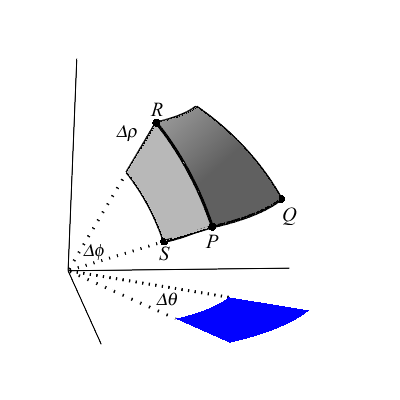
\includegraphics[trim=0.5cm 1cm 1.5cm 1cm, clip]{11_8_Spherical_volume_element}}
  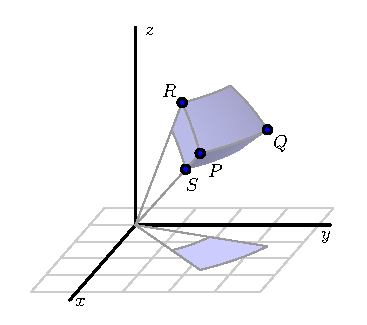
\includegraphics{figures/fig_11_8_spherical_box.eps}
\end{center}
\caption{A spherical box.}
\label{F:11.8.Spherical_Vol_Element}
\end{minipage} \hspace{0.5in}
\begin{minipage}{2.5in}
\begin{center}
%\resizebox{!}{2.4in}{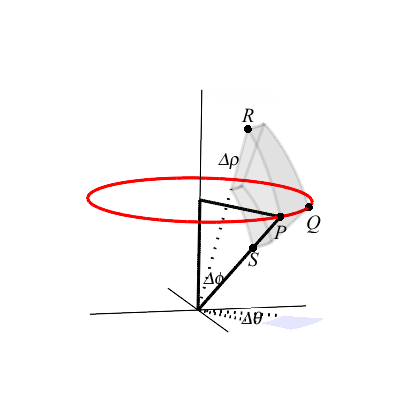
\includegraphics[trim=1.5cm 1.5cm 1.5cm 1.5cm, clip]{11_8_Spherical_volume_element_b}}
  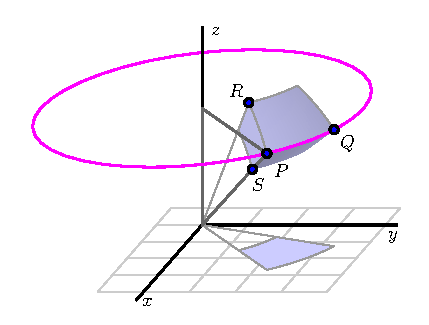
\includegraphics{figures/fig_11_8_spherical_volume.eps}
\end{center}
\caption{A spherical volume element.}
\label{F:11.8.Spherical_Vol_Element_b}
\end{minipage}
\end{center}
\end{figure}
%crop graphics in animate trim=<left> <bottom> <right> <top>, clip with includegraphics
    \ba
        \item What is the length $|PS|$ in terms of $\rho$? 
        %$\Delta \theta$, $\Delta \phi$, $r_1$, $r_2$, $\theta_1$, $\theta_2$, $\phi_1$, and $\phi_2$?

    \item What is the length of the arc $\overset{\frown}{PR}$? (Hint: The arc $\overset{\frown}{PR}$ is an arc of a circle of radius $\rho_2$, and arc length along a circle is the product of the angle measure (in radians) and the circle's radius.)


    \item What is the length of the arc $\overset{\frown}{PQ}$? (Hint: The arc $\overset{\frown}{PQ}$ lies on a horizontal circle as illustrated in Figure \ref{F:11.8.Spherical_Vol_Element_b}. What is the radius of this circle?)


    \item Use your work in (a), (b), and (c) to determine an approximation for $\Delta V$ in spherical coordinates.


    \ea

\end{activity}
\begin{smallhint}

\end{smallhint}
\begin{bighint}

\end{bighint}
\begin{activitySolution}
   \ba
    \item The length $|PS|$ is just $\Delta \rho$. 

    \item This arc is a fraction $\frac{\Delta \phi}{2 \pi}$ of the entire circle of radius $\rho_2$, so its length is
\[\left(\frac{\Delta \phi}{2\pi}\right)(2 \pi \rho_2) = \rho_2 \Delta \phi.\]


    \item The radius of the on which the arc $\overset{\frown}{PQ}$ lies is $\rho_2 \sin(\phi_2)$, so the length of the arc $\overset{\frown}{PQ}$ is  \[\left(\frac{\Delta \theta}{2\pi}\right)(2 \pi \rho_2 \sin(\phi_2)) = \rho_2 \sin(\phi_2) \Delta \theta.\]


    \item The results from the previous parts of this activity show that
\[\Delta V \approx \rho_2^2 \sin(\phi_2) \Delta \rho \Delta \phi \Delta \theta.\]
Letting $\Delta \rho$, $\Delta \phi$, and $\Delta \theta$ go to 0 gives us
\[dV = \rho^2 \sin(\phi) \, d\rho \, d\phi \, d\theta.\]

    \ea
\end{activitySolution}
\aftera
